%
% $Id: $
%

%\documentclass[times,10pt,twocolumn]{article}
%\documentclass[times,12pt]{article}
\documentclass[a4paper,11pt]{article}
\usepackage[utf8]{inputenc}
\usepackage{times}


\newcommand{\finejercicio}{
  \begin{footnotesize}
    [Al terminar el ejercicio es recomendable hacer \texttt{commit} de los ficheros modificados]
  \end{footnotesize}
}

\newcommand{\finpractica}{
  \begin{footnotesize}
    [Al terminar la práctica, realiza un \texttt{push} para sincronizar tu repositorio GitHub]
  \end{footnotesize}
}

%\documentstyle[times,art12,format/latex8]{article}

\usepackage{url}

\usepackage{fullpage}
\usepackage{subfigure}
\usepackage{amssymb}
\usepackage{amsmath}
\usepackage{psfrag}
\usepackage{epsfig}
\usepackage{graphicx}
\usepackage{graphics}

% COMMENTS (optional argument is author of comment)
\newcommand{\comments}[2][?]{
  \begin{quote}
    \textbf{Comment (#1):} {\em #2}
  \end{quote}
  }
%% Uncomment this line to remove comments
%\renewcommand{\comments}[2][?]{}


%-------------------------------------------------------------------------
% take the % away on next line to produce the final camera-ready version
\pagestyle{empty}

%-------------------------------------------------------------------------
\begin{document}


\title{Práctica 6 - Sesión SIP \emph{peer-to-peer}}
\author{Protocolos para la Transmisión de Audio y Vídeo en Internet}
\date{Versión 8.0 – 3.11.2017}

%\author{Gregorio Robles y Jesús M. González Barahona \\
%  grex@gsyc.urjc.es \\
%  Grupo de Sistemas y Comunicaciones \\
%  Universidad Rey Juan Carlos
%}

%\date{Febrero 2010}

\maketitle
\thispagestyle{empty}

%\maketitle
%\tableofcontents
%\newpage

%-------------------------------------------------------------------------

Nota: Esta práctica se puede entregar para su evaluación como parte de la nota de prácticas, pudiendo obtener el estudiante hasta 0,7 puntos. Para las instrucciones de entrega, mira al final del documento.

\section*{Introducción}

Esta práctica tiene como objetivo implementar dos programas Python,
de manera que se pueda realizar una sesión SIP como la que se
muestra en la figura\footnote{Nota que en la figura las respuestas SIP están en 
mayúsculas para mejorar su lectura; en tu implementación deberían seguir el 
estándar con sólo la primera letra mayúscula}:

\begin{center}
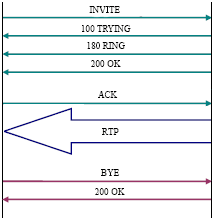
\includegraphics{figs/sip-invite.png}
\end{center}

En esta sesión:

\begin{itemize}
  \item No habrá ni servidor de registro ni \emph{proxy}. La comunicación será \emph{peer-to-peer} (directa entre dos UAs\footnote{UA: User Agent. Un UA se compone de un cliente y un servidor, aunque en esta práctica -por simplificación- cada UA tendrá sólo uno de los dos.}).
  \item El UA de la izquierda constará exclusivamente de la parte cliente. Esta parte será la que inicie la sesión con un \texttt{INVITE} y la cierre con un \texttt{BYE}.
  \item El UA de la derecha constará exclusivamente de la parte servidora. Esta parte será la que envíe el audio vía RTP al cliente.
\end{itemize}


\section*{Objetivos de la práctica}

\begin{itemize}
  \item Implementación de una conversación de audio iniciada con SIP.
\end{itemize}

\section*{Conocimientos previos necesarios}

\begin{itemize}
  \item Nociones de SIP (las de clase de teoría)
  \item Funcionamiento de \texttt{wireshark}.
\end{itemize}

Tiempo estimado: 10 horas

\section*{Creación de repositorio para la práctica}

Con el navegador, dirígete al repositorio \texttt{ptavi-p6} en la cuenta del profesor en GitHub\footnote{\url{http://github.com/gregoriorobles/ptavi-p6}} y realiza un \texttt{fork}, de manera que consigas tener una copia del repositorio en tu cuenta de GitHub. Clona el repositorio que acabas de crear a local para poder editar los archivos. Trabaja a partir de ahora en ese repositorio, sincronizando los cambios que vayas realizando.

 Como tarde al final de la práctica, deberás realizar un \texttt{push} para subir tus cambios a tu repositorio en GitHub. En esta práctica, al contrario que con las demás, se recomienda hacer frecuentes \texttt{commits}, pero el \texttt{push} al final.


\section*{Parte cliente}

El cliente ha de ejecutarse de la siguiente manera:
\begin{verbatim}
  $ python3 client.py metodo receptor@IPreceptor:puertoSIP
\end{verbatim}

donde \emph{metodo} será un método SIP, \texttt{receptor@IPreceptor:puertoSIP}
será el login, la IP y el puerto\footnote{En el mundo ``real'', el puerto sería 
el puerto de SIP por defecto, el 5060, ya que sólo puede haber un UA activo
por máquina - si arrancas otro Ekiga cuando hay uno ya lanzado, no podrás.
Sin embargo, como tenemos dos UAs en la
misma máquina, hemos de especificar un puerto para que no se ``pisen''.}
al que se dirige el mensaje.

Por ejemplo:
\begin{verbatim}
  $ python3 client.py INVITE batman@193.147.73.20:5555
  $ python3 client.py BYE robin@193.147.73.20:5555
\end{verbatim}

En caso de no introducir el número de parámetros correctos o de error en los mismos, el programa debería imprimir siempre por pantalla:

\begin{verbatim}
  Usage: python3 client.py method receiver@IP:SIPport
\end{verbatim}

\subsection*{Peticiones SIP}

  \begin{itemize}
    \item INVITE sip:receptor@IP SIP/2.0

    Mediante este método, se indica que queremos iniciar una conversación con el receptor con dirección receptor en la máquina dada por la IP (que puede ser 127.0.0.1).

    \item ACK sip:receptor@IP SIP/2.0

    Método de asentimiento. No se pasará al programa \texttt{client.py} como parámetro desde
la \texttt{shell}, ya que se enviará de manera automática una vez se hayan recibido las respuestas \texttt {100 Trying}, \texttt{180 Ring} y \texttt{200 OK} de la parte servidora tras hacerle un INVITE.

    \item BYE sip:receptor@IP SIP/2.0

    Mediante este método se indica que queremos terminar una conversación con el receptor con dirección receptor en la máquina dada por la IP (que puede ser 127.0.0.1). Se deberá llamar, una vez haya acabado el \emph{streaming} de audio vía RTP desde el lado servidor.

  \end{itemize}


\section*{Parte servidora}

El servidor ha de ejecutarse de la siguiente manera:
\begin{verbatim}
  $ python3 server.py IP puerto fichero_audio
\end{verbatim}

Por ejemplo:
\begin{verbatim}
  $ python3 server.py 127.0.0.1 5555 cancion.mp3
\end{verbatim}

En caso de no introducir el número de parámetros correctos o de error en los mismos (se ha de comprobar si existe el fichero de audio), el programa debería imprimir:
\begin{verbatim}
  Usage: python3 server.py IP port audio_file
\end{verbatim}

En caso de no haber error al arrancar, el servidor imprimirá por pantalla:
\begin{verbatim}
  Listening...
\end{verbatim}

\subsection*{Códigos de respuesta}

   \begin{itemize}
     \item \texttt{SIP/2.0 100 Trying}: al recibir un INVITE.
     \item \texttt{SIP/2.0 180 Ringing}: al recibir un INVITE.
     \item \texttt{SIP/2.0 200 OK}: en caso de éxito.
     \item \texttt{SIP/2.0 400 Bad Request}: si la petición está mal formada.
     \item \texttt{SIP/2.0 405 Method Not Allowed}: si se manda en la petición cualquier otro método diferente de INVITE, BYE o ACK.
   \end{itemize}

Nota: Para simplificar la práctica, se enviará en un único mensaje la respuesta \texttt{SIP/2.0 100 Trying}, \texttt{SIP/2.0 180 Ringing} y \texttt{SIP/2.0 200 OK}.

\subsection*{Envío RTP}

El envío RTP se realizará mediante el programa \texttt{mp32rtp}\footnote{En el repositorio se encuentra un binario precompilado para entornos Debian GNU/Linux, entre los que se encuentran Ubuntu, el sistema operativo utilizado en los laboratorios docentes.}. La forma de ejecutar el programa \texttt{mp32rtp}, una vez se le haya dado permisos de ejecución con \emph{chmod}, es indicando la dirección IP y el puerto del receptor y redirigirle una canción en formato MP3:

\begin{verbatim}
  ./mp32rtp -i direccionIP -p puerto < cancion.mp3
\end{verbatim}

De esta manera, para enviar un \emph{stream} a \emph{localhost} al puerto 23032, la línea de \texttt{shell} que se ha de ejecutar es:

\begin{verbatim}
  ./mp32rtp -i 127.0.0.1 -p 23032 < cancion.mp3
\end{verbatim}

Para ejecutar instrucciones de \texttt{shell} desde Python, se puede utilizar algunos métodos del módulo \texttt{os}, en particular \texttt{system()}. El parámetro que se le pasa a \texttt{system} 
es lo que se ejecutaría como si fuera la \texttt{shell}.

Un ejemplo del código sería el siguiente\footnote{Cuando se copia de un PDF
a un editor de texto, puede que algunos caracteres, en especial las comillas
no sean las ``correctas'' y nos dé un error. Tenlo en cuenta.}:

\begin{verbatim}
  import os

  # aEjecutar es un string con lo que se ha de ejecutar en la shell
  aEjecutar = 'mp32rtp -i 127.0.0.1 -p 23032 < ' + fichero_audio 

  print("Vamos a ejecutar", aEjecutar)
  os.system(aEjecutar)
\end{verbatim}

Nótese que \texttt{fichero\_audio} es uno de los parámetros que se le pasa al servidor al ejecutarse. {\bf Nota: Como en esta práctica no se hace uso de SDP para 
describir la sesión, se utilizará la IP 127.0.0.1 y el puerto 23032 como
destino del envío}.

\section*{Captura}

Una vez terminada la práctica, se pide que se realice una captura de un
establecimiento de llamada, el envío RTP de audio y la finalización de
la llamada. 

La captura original se filtrará para que sólo incluya los paquetes
SIP y los tres primeros y tres últimos paquetes RTP con audio.

La captura filtrada resultante se guardará en el fichero \texttt{invite.libpcap}
y se subirá al repositorio.


\section*{Fecha y modo de entrega}

La entrega de práctica se deberá hacer antes del lunes 27 de noviembre de 2017 a las 23:55. Para entonces, se debe tener un repositorio git en GitHub con: 

    \begin{itemize}
        \item 2 módulos Python y la captura realizada con \texttt{wireshark}:
    \begin{itemize}
      \item \texttt{server.py}
      \item \texttt{client.py}
      \item \texttt{invite.libpcap}
    \end{itemize}
    \item 5 ficheros adicionales (además de \texttt{.git}): \texttt{README.md}, \texttt{LICENSE}, \texttt{check-p6.py}, \texttt{mp32rtp} y \texttt{.gitignore}.
\end{itemize}

Se han de tener en cuenta las siguientes consideraciones:
\begin{itemize}
  \item Se valorará que al menos haya diez \emph{commits} realizados en al menos dos días diferentes.
  \item Se valorará que la captura esté bien filtrada y sólo contenga los paquetes que se indican en el guión.
  \item Se valorará que el código entregado siga la guía de estilo de Python (véanse PEP8 y PEP257).
  \item Se valorará que los programas se invoquen correctamente y que muestren los errores correctamente, según se indica en el enunciado de la práctica.
\end{itemize}

Se puede comprobar la correcta entrega de la práctica utilizando el programa \texttt{check-p6.py}. Este programa se ejecuta desde la línea de comandos de la siguiente manera:
\begin{verbatim}
  $ python3 check-p6.py login_github
\end{verbatim}


donde \texttt{login\_github} es tu nombre de usuario en GitHub.



%-------------------------------------------------------------------------
%\nocite{ex1,ex2}
%\bibliographystyle{format/latex8}
%\bibliography{libresoft}

\end{document}
